\documentclass[a4paper,
fontsize=11pt,
%headings=small,
oneside,
numbers=noperiodatend,
parskip=half-,
bibliography=totoc,
final
]{scrartcl}

\usepackage{synttree}
\usepackage{graphicx}
\setkeys{Gin}{width=.4\textwidth} %default pics size

\graphicspath{{./plots/}}
\usepackage[english]{babel}
\usepackage[T1]{fontenc}
%\usepackage{amsmath}
\usepackage[utf8x]{inputenc}
\usepackage [hyphens]{url}
\usepackage{booktabs} 
\usepackage[left=2.4cm,right=2.4cm,top=2.3cm,bottom=2cm,includeheadfoot]{geometry}
\usepackage{eurosym}
\usepackage{multirow}
\usepackage[english]{varioref}
\setcapindent{1em}
\renewcommand{\labelitemi}{--}
\usepackage{paralist}
\usepackage{pdfpages}
\usepackage{lscape}
\usepackage{float}
\usepackage{acronym}
\usepackage{eurosym}
\usepackage[babel]{csquotes}
\usepackage{longtable,lscape}
\usepackage{mathpazo}
\usepackage[flushmargin,ragged]{footmisc} % left align footnote

\usepackage{listings}

\urlstyle{same}  % don't use monospace font for urls

\usepackage[fleqn]{amsmath}

%adjust fontsize for part

\usepackage{sectsty}
\partfont{\large}

%Das BibTeX-Zeichen mit \BibTeX setzen:
\def\symbol#1{\char #1\relax}
\def\bsl{{\tt\symbol{'134}}}
\def\BibTeX{{\rm B\kern-.05em{\sc i\kern-.025em b}\kern-.08em
    T\kern-.1667em\lower.7ex\hbox{E}\kern-.125emX}}

\usepackage{fancyhdr}
\fancyhf{}
\pagestyle{fancyplain}
\fancyhead[R]{\thepage}

%meta
%meta

\fancyhead[L]{E. Blumer \& K. Schuldt \\ %author
LIBREAS. Library Ideas, 26 (2014). % journal, issue, volume.
\href{http://nbn-resolving.de/urn:nbn:de:kobv:11-100222616
}{urn:nbn:de:kobv:11-100222616}} % urn
\fancyhead[R]{\thepage} %page number
\fancyfoot[L] {\textit{Creative Commons BY 3.0}} %licence
\fancyfoot[R] {\textit{ISSN: 1860-7950}}

\title{\LARGE{Urban Revitalization, Gentrification, and the Public Library: The Case of Lausanne, Switzerland}} %title %title
\author{Eliane Blumer \& Karsten Schuldt} %author

\setcounter{page}{19}

\usepackage[colorlinks, linkcolor=black,citecolor=black, urlcolor=blue,
breaklinks= true]{hyperref}

\date{}
\begin{document}

\maketitle
\thispagestyle{fancyplain} 

%abstracts
\begin{abstract}
Gentrification -- a process of replacement of a poorer population in an
urban neighborhood with a richer one and the change of the looks of this
respective neighborhood -- has become a widespread topic of societal
debates in recent years. This process is linked to public art and
cultural activities, and sometimes triggered with projects of urban
revitalization by the respective cities. Public libraries are part of
this process and they are used in the concepts of urban revitalization
as well as institutions for public culture. This puts them in an uneasy
position: thus, libraries also become part in processes of the repulsion
of socially vulnerable groups. The text will discuss the current
position of public libraries in respect to gentrification, using some
incidents in the city of Lausanne, Switzerland, as a case study.
\end{abstract}

%body
Should public libraries engage in projects for urban revitalization and
if so, in which role? What, if this revitalization leads to
gentrification, social segregation and displacement of open drug users
or other socially vulnerable groups? This text will try to deal with
these issues.

In recent years, discussions and social movements around the question of
urban revitalization, the \enquote{right to the city} and/or
gentrification have emerged with a remarkable vitality in Europe,
Australia, and North America. (Lees, Slater \& Wyly 2008) More often
than not, art and cultural projects became part of these controversies.
Sometimes, libraries happen to be used as part of the revitalization
attempts of urban spaces as well. This is what happens in Lausanne,
Switzerland and this text will use Lausannes situation -- both the
neighborhood of the Flon and the Place de la Riponne -- as case study
for this phenomenon. But: the dealt issues one can find in this text are
not limited to Lausanne. Big cities in Europe and the Global North keep
growing, almost all of them have strategies to govern these growth
processes. In an increasing number of cities those changes lead to
social conflicts, some, like the protests in Berlin, New York or San
Francisco with a widespread coverage, but most of them only with local
visibility. Either way, public libraries in those cities can't ignore
upcoming conflicts around urban revitalization and/or gentrification,
because they are affected by changes and are part of them at the same
time.

The remaining text is structured as follows. (1) It discusses the
gentrification process and its importance in recent urban development by
introducing a three phase model. (2) Afterwards, text continues with a
greater insight in Lausannes situation, especially to the neighborhoods
of Flon and Riponne. The text ends (3) with an outline of the role of
public libraries and proceed with a formulation of proposals for a
further discussion in the library community.

\section{Urban revitalization, gentrification, and the
displacement of the socially
excluded}\label{urban-revitalization-gentrification-and-the-displacement-of-the-socially-excluded}

In recent years, gentrification has become one of the pressing topics of
social uproar in different countries, especially in big cities and
metropolises. (Holm 2014, Prince 2014, Andres \& Grésillon 2013, Naegler
2012, DeSena 2009, Lees, Slater \& Wyly 2008) Starting as a term used in
urban sociology and by political activists it is now used as a common
term in newspapers, everyday discussions and political programs. In some
cities like Berlin or Hamburg gentrification seems to be a social
development which concerns nearly everyone. As this former scientific
term becomes more and more widespread, the meaning of gentrification
broadens up. It is sometimes an expression of a feeling of an unwanted
shift in the urban landscape and culture, not always grounded in
empirical facts. And it is a postmodern concept, as usually those people
which seem to drive gentrification are the same people who want to limit
negative consequences of this urban change.

Gentrification is at first a term for a tremendous rise of rents. Sooner
or later, a change in the population living in certain urban
neighborhoods happens, as it seems as if the more poor and more
vulnerable population of those neighborhoods is gradually driven out of
the gentrified area. But it is more than that. Gentrification also
describes the change of the culture, the social structure, and the
lifestyle in one neighborhood, usually marked by the closure of the
infrastructure used by poor people for their everyday life -- like cheap
supermarkets or stores, basic pubs and so on -- and a rise of the number
of cafés, restaurants, shops and infrastructure for a better paying
clientele at the same time. This is not just a question of prices, it is
also a question of different cultures, whereas the new bars and shops
usually seem to be oriented towards a clientele that is more interested
in culture, health and alternative lifestyles.

But: not all of those changes are seen as a bad thing, not everybody
conceives them as negative. For instance, more art, a wider range of
eating offers (Stock 2013) or a less violent street live (DeSena 2009)
are quite often described as a good outcome of the processes known as
gentrification. Most often these processes are linked to the
disappearing of visible illegal behavior. Groups of public visible drug
users are often among the first ones being targeted by those changes and
tend to disappear quite fast. For instance, the fight of local stores
and neighborhood groups against a public injection room marked, in a
way, also the beginning of the active gentrification of the
\enquote{Schanzenviertel} in Hamburg. (Naegler 2012)

Still, there are other terminologies used to describe these process,
especially when those changes are planned. Then they are discussed as
\enquote{urban renewal} or \enquote{urban revival}. Usually,
\enquote{urban revival} is fostered by the cities itself, but also by
organizations commissioned by the cities too -- like the
\enquote{Quartiersmangement} in Berlin or the \enquote{Stadterneuerungs-
und Stadtentwicklungsgesellschaft Hamburg} (Naegler 2012) -- or private
investors. Lees, Slater and Wyly (Lees, Slater \& Wyly 2008) point out
that cities and investors usually avoid the term gentrification by
choice, even outright disputing the legacy of the term. They understand
gentrification -- or, in their words, \enquote{urban development} -- as
a favorable process, providing much more positive than negative effects
for the respective neighborhoods and their inhabitants.

These processes are even more complex, as they sometimes seem to be
triggered by groups who explicitly don't want to displace poor and
socially excluded people, but try to live alternative lifestyles -- like
artists, students or member of different subcultures -- or even people
who contest the current economic system, such as left-radical centers
like the \enquote{Rote Flora} in Hamburg (Naegler 2012). At the same
time, not every project of urban revival succeeds, not every
neighborhood that could become gentrified will do so, and
simultaneously, other areas of the cities become less gentrified or even
impoverished.

\subsection{A Model of Gentrification}\label{a-model-of-gentrification}

A widely used theoretical model to explain gentrification in the context
of urban sociology was introduced by Andrej Holm.\footnote{Holm gained
  somewhat of prominence right at the time, when gentrification as a
  term became known outside of sociology and political activism, when in
  2007 he was -- together with three other people -- arrested on behalf
  of the Federal Attorney General of Germany and accused of membership
  of a left-wing, terrorist group called \enquote{militante gruppe}. In
  the progress of the case it became clear, that authorities had added
  Holm to the group because both used the terms \enquote{gentrification}
  and \enquote{precarization} in their texts. The detention of Holm
  became a political issue when several international scientists signed
  a declaration for Holm. No charges against Holm were pressed, but this
  story became one of the starting points for the popularity of the term
  \enquote{gentrification} in the German public.} His model will be used
in this text.

Gentrification, as it is described in Holms model, is triggered first
and foremost by the interests of homeowners to rise the rents of their
housings up until the point where they get the most profit out of them.
This can, but does not have to, include the massive renovation of
housing and infrastructure that should support the quality of housing.
Every housing that is up for rental has a potential rent, which is
defined by the quality of housing, by the infrastructure and culture
around the housing, by the whole renting market of a city, by interests
and financial potentials of the possible renters, but also by political
guidelines, zoning and policies. Homeowners tend to try to exploit those
potential rents -- or, in other words, close the \enquote{rent gap} --,
but are usually not able to max out those rents in a short time, because
a rise of rents is not only in their hands. Usually, they try to get the
potential rents in cases of new tenants.\footnote{This doesn't mean that
  homeowners always estimate the potential rents correctly. Sometimes,
  they overestimate the demand or financial possibilities of potential
  tenants. This seems to be the case in Zürich, where recently a growing
  number of high-priced new apartments have problems to find new
  tenants, although the demand for apartments is still high. (Stadt
  Zürich Präsidialdepartement 2014)}

Gentrification is understood as a process, not a static situation. As
every process it can be interrupted, slow down or change direction.
Nevertheless, Holm (2011) presents a model of gentrification that
describes three distinct phases.

\begin{itemize}
\item
  Phase 1: An urban area is suited for gentrification. Rundown building
  stock exists in an acceptable quality or can be renovated towards such
  quality, rents are low, usually there are a great number of vacant
  spaces or shops. Typically, those areas are part of the inner city or
  nearby, with public transportation already in place. The number of
  people looking for a relocation into the inner city is rising.
\item
  Phase 2: \enquote{Pioneers} move into the area, usually because of
  cheap rents and/or the search for free space to try alternative forms
  of lifestyle. Those alternative styles can include political activism,
  art, alternative forms of personal live and the like. Quite often
  those pioneers combine high cultural and social capital with little
  economic capital, e.g.~artists who do art, but doesn't gain much
  wealth from selling it or students, which study and accumulate
  cultural and educational capital without making money out of this
  capital, yet. The look of the neighborhood changes: street cafés, art
  galleries, diverse forms of restaurants and shops tailored to the
  pioneers emerge. Over the time, rents tend to rise, old shops and
  infrastructures tend to disappear and the population changes as well.
  Usually, the most vulnerable groups tend to disappear from the
  landscape.
\item
  Phase 3: In the third phase of gentrification, the culture of the
  everyday life has changed completely. New tenants pay high rents,
  usually the building stock is renovated and kept in high quality. The
  street life is dominated by people from the higher social classes and
  the infrastructure is tailored to their demands. For instance,
  discounter chains have vanished, more expensive organic grocery stores
  have emerged. The rhythms of the neighborhood have changed according
  to the inhabitants, e.g.~were bars tailored for students and young
  artist tend to be open until the early morning, bars in highly
  gentrified areas tend to close early, as most of the inhabitants tend
  to work in \enquote{normal} nine-to-five jobs. Not only poor people
  have left the neighborhood, but pioneers of the second phase did also.
  Sometimes they have become older and richer, like students who
  finished their education, entered the job market and settled with
  children. Although most of the inhabitants tend to have liberal or
  leftist political views, and sometimes engage in favor of alternative
  lifestyles, most of those have vanished or have been incorporated into
  the picture of the neighborhood, without being actually
  lived.\footnote{Hae (2012) analyzed those contradictory changes in New
    York nightlife, when parts of the city moved from the second to the
    third phase of gentrification and described it as a process of
    becoming \enquote{boring} (DeSena 2009), while still trying to
    profit from the picture of a highly vitalized city life fostered in
    the first and second phase: \enquote{As the city has experienced
    gentrification throughout the last three decades, \enquote{noisy}
    and \enquote{boisterous} nightlife businesses in gentrifying
    neighborhoods, including bars and lounges as well as dance clubs,
    have been censured as the number one enemy of \enquote{quality of
    life} in these neighborhoods due to their nuisance effects.
    Ironically, this process has gone on even as the real estate sector
    trumpeted and marketed the profile of nightlife in these communities
    as a sign of neighborhood vibrancy in order to boost property
    values. That is, nightlife establishments and their cultural
    elements have been one of the important catalysts for gentrification
    of the very neighborhoods in which the presence of these businesses,
    later, have been intensely contested by groups of gentry that have
    moved here.} (Hae 2012, 2)}
\item
  A possible phase 4 of hyper-gentrification is only suggested by Holm
  (2011): Sometimes neighborhoods or parts of them evolve into a phase
  of hyper-gentrification, where those areas become home of much richer
  people, with an international focus, usually marked by luxury
  apartment buildings. They become part of what may be better termed as
  \enquote{global cities}: a network of places, interconnected,
  depending on the city functions, like the amassing of cheap but
  talented labor, and highly specialized small businesses belonging to
  the tertiary sector, but without a real touch to the rest of the
  neighborhoods they are in. (Sassen 2001)
\end{itemize}

Holm (Holm 2011, Holm 2014) emphasizes that most of the social conflicts
surrounding gentrification tend to happen in the second phase (see
e.g.~DeSena 2009, Prince 2013), although the real problems of expulsion
and exclusion are to be found in the third phase. The moving in of
pioneers, openings of street cafés as well as organic grocery stores, or
the first \enquote{sightings} of tourists don't pose a threat to the
more vulnerable inhabitants; but rising costs of rent and living do. But
sometimes such visible changes are necessary as catalyst for protest
against gentrification to happen, because the conflicts then would
become concrete. (Holm 2014)

Gentrification usually is a longtime process of replacing a population
with a significant much richer and more powerful population, starting
with the most vulnerable. For instance, in Berlin it is usually not the
rich who follow when the poor move out of a gentrified area or
apartment, but slightly less poorer people, which are then followed by
even a little more richer ones and so on. (Holm 2014, Bonal \& Gude
2014) But still, when gentrification starts to enter the second phase in
one area, the number of \enquote{gentrification moments} (Prince 2014)
starts to rise. Today, people and activists seem to be alerted to such
changes and moments, compared to some years ago.

\subsection{Culture and Gentrification}\label{culture-and-gentrification}

An open issue -- both in the scientific and the societal discussion --
is still the connection between culture and gentrification. Usually the
opening of cultural places like art galleries is seen as a trigger of
gentrification. This is consistent with Holms 3-phase-model: Pioneers
moving in a previously impoverished area mark the beginning of the
second phase. Artists and people with high cultural assets are seen as
such pioneers, which doesn't mean, that they always intend to be such
pioneers. Many a time, they specifically try to reject that role. They
are the ones which try to bring more aspects of cultural life to such an
area, but don't want to repulse people. Sometimes they try to reflect
their situation, sometimes they strictly reject it.\footnote{For
  instance, when Christina M. Heinen (Heinen 2013) did her research on
  the musical cultures in Berlin-Neukölln - one of Berlin's
  gentrification areas - in 2008 to 2010, she received a strict
  rejection for an interview from one musician, because she, as a
  researcher, was seen as part of the gentrification process and the
  musician wished to have no part in this: \enquote{At first the field
  researchers arrive, then the diggers.} (Heinen 2013, 30. \enquote{Erst
  kommen die Feldforscher, dann die Bagger.})}

The idea of a conjunction between cultural activities and gentrification
is a result of the discussion about a \enquote{creative class}. This
creative class, it is believed particularly in institutions which are in
the position to plan the development of cities, is a term for people
doing \enquote{creative} work, whereby this includes quite different
professions, from artists to marketing specialists, from actors and
writers to architects and entrepreneurs. Such a creative class should
need each other to be productive, for example architects and
entrepreneurs should need the stimulus of art and theaters as well as
the concentration of a busy urban live. Although, empirical facts about
the realities of the \enquote{creative class} are ambiguous, more and
more city officials got convinced -- with the help of academic or
economic advisors --, that they need more members for flourishing their
cities. (Terrin 2012) Hence, they try to stimulate urban revitalization
with the help of creative endeavors. Art galleries and little theaters
are funded, sometimes only on a short term basis, festivals of different
forms are invited or invented, special regulations for pubs, like longer
opening hours or the relaxation of the enforcement of regulations, are
put in place, museums are opened, and even libraries are included into
the strategies for urban redevelopment.

At the same time, pioneers are more inclined to do such creative work on
their own, for instance by opening up art galleries, pubs and other
entrepreneurial ideas their like to start up with, including organize
cultural events. It is not clear, if any of this activities leads
directly to gentrification. Schuetz (Schuetz 2013) points out that art
galleries in European and US-American cities, when they are established
or move, do not follow the movements of gentrification, but rather
historical patterns of their respective city and orient themselves on
already existing galleries and museums. On the other hand, nearly every
area that was affected by gentrification in the last decades possessed a
share of some forms of cultural infrastructure. (Terrin 2012)

While the data are not much coherent and even though not all forms of
cultural activity lead to gentrification, it is not possible to talk
about gentrification or urban revitalization without reflecting on
cultural activities, particularly those tailored not just to a small
elite but to a wider audience, like for instance libraries.

\section{The case of Lausanne}\label{the-case-of-lausanne}

Lausanne, which will be used here as the case study object, is the
fourth largest city of Switzerland, with about 130.000 inhabitants and
the second biggest one in the French speaking part of this country.
However, compared to cities in the neighboring countries, it is a major
city with a rather average size. It is the capital of the Canton of Vaud
and among other things, home to the Swiss Federal Institute of
Technology in Lausanne, the University of Lausanne as well as the
International Olympic Committee. Situated at the Lac Léman and at the
border of Switzerland and France, Lausanne today is known as the main
spot for the clubbing scene in the area, as well as a center for
cultural events. It is, compared to other Swiss municipalities, quite a
young and busy city with a high number of young people and students.

\subsection{From deserted warehouses to Flon-Flon, from Flon-Flon to
Flon}\label{from-deserted-warehouses-to-flon-flon-from-flon-flon-to-flon}

The example of the Place de la Riponne in Lausanne, which this case
study is focusing on, has an important predecessor in the city, the area
of Flon. The Flon is an area, highly gentrified today, only one metro
station away from the Riponne. From the 1950s onwards this was a
rundown, post-industrial district, situated in the middle of the city,
but in a small valley, some meters below the city level and filled only
with partly used warehouses. Subject to different plans for
revitalization and societal conflicts (Zuppinger 2012), it became a
center for alternative culture in Switzerland under the name
\enquote{Flon-Flon}. Since last century turn, the Flon increasingly
became the \enquote{in quarter} of Lausanne for another kind of young,
urban, but not always alternative or \enquote{hip} groups of people.
Although one of the places for nightlife in the city, today it seems
like a big outdoor commercial-zone in contrast to the more bottom-up
culture of the 1990s. Whereas the transformation in the 1990s was made
possible by the conflicts of the years before, but impelled by people
that could be described as pioneers according to Holms model, the turn
after 2000, enforced by the city and the main proprietor of the Flon,
can be linked to the third phase.

Until the 1950s, the Flon was a port on the way to the nearby Lac Léman,
used primarily for industrial goods. Most of the industry situated in
the Flon left the area in course of the years. This was consistent with
movements one could also observe in other European cities, were the
actual industrial production got sourced out. As in other cities too,
this left brownfields of slowly deteriorating buildings. Every city had
to deal with its brownfields. Some, most renowned Detroit (2012), left
most of this area open in case the city is able to change their current
course of urban development. Other cities like Marseille tried to
reanimate their usable area by installing cultural institutions (Andres
\& Grésillon 2013) or, like Berlin in the 1990s, left the horizon of
their not used space quite open and developed a culture of short-term
uses (Andres \& Grésillon 2013). In this context, Lausannes situation is
specifically marked by a constant shortage of housing, most notably
affordable ones. This is consistent with the situation of most larger
Swiss cities. (Andres \& Grésillon 2013) Therefore the Flon, as an only
rarely used space next to the city center, was for decades a subject to
plans for different uses. Nevertheless, none of these plans bear fruit.
In 1984, the city together with the main real estate of the Flon,
proposed a project for a city interstate, which would have included the
demolition of the existing buildings. The plan was an example of plans
for automotive cities. While some of these plans were implemented in
other cities, in Lausanne a group of concerned citizen formed the group
\enquote{Groupe Action Urbanisme}, which took to the streets against
such schemes. Later, this group and other citizens formed the
\enquote{Association pour un aménagement harmonieux du Flon} (APAHF,
Coalition for a harmonic development of the Flon). For the next decades,
the actions of the APAHF influenced to evolution of the Flon.

APAHF preferred a development of the city they called
\enquote{l'urbanisme du rêve} (urbanism of dreams or utopian urbanism),
which aimed to include interests and participation of different groups
and had the vision of a more lively city. (Zuppinger 2012\footnote{This
  book was written as a retrospective of one of the most involved member
  of the APAHF. Although it includes an immense batch of otherwise
  unknown sources, it surely presents the position of the APAHF in a
  good light. Nevertheless, the influence of the group should not be
  underestimated, as they won popular votes in the city and had a high
  publicity in the public debate.}) In 1986, APAHF won a popular vote
against this plan. Such popular votes are common in Switzerland on such
vast projects. The city had zoned the Flon as \enquote{industrial site},
which meant, that other ways of utilization like flats or commercial
projects were not possible as long term alternatives. This situation
left the real estate in an uneasy position. There was little industry to
settle there. A part of the Flon became a carhouse for the public buses
in Lausanne, another building at the edge of the Flon was turned into a
shopping center. But most of the old warehouses were rented out in the
years ahead for short term leases like galleries, bars, alternative
clubs et cetera. In the early 1990s, the Flon had become a center for
alternative cultures, mixing interests of artists, political activists
and mostly small shop owners, above all galleries, second hand shops and
bookshops. (Andres \& Grésillon 2013) In other words: the Flon moved
into the second phase of gentrification, although tenants were only
slightly affected, as there were only a small number of flats on this
site too. This development was only possible because of the Flons vague
status then, leading to an open attitude by the real estate, which gave
out short-term rent, and the city which didn't impose another
development plan of the Flon.

Starting in 1989, the commercial center mentioned above, published a
magazine, \enquote{gazette du flon}, which in the first year was used as
a marketing tool for the center. After the first year, the magazine was
taken over by another editorial team and focused on the Flon itself.
Nevertheless, in the third number of the Gazette, still published by the
center, an article that dealt with the emerging art scene first can be
found there. (Anonymous 1989) In the short time between the popular vote
in 1986 and 1989, the image of the Flon had changed completely.

\begin{figure}[htbp]
\centering
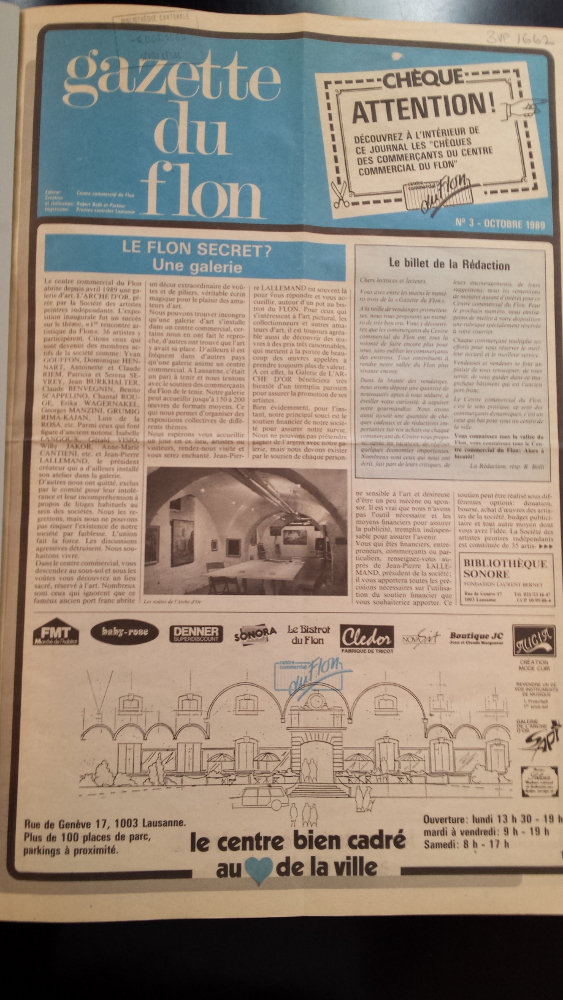
\includegraphics{img/BlumerSchuldt01.jpg}
\caption{The 1989 issue of the \enquote{gazette du flon} mentioned above
with the first article about the galleries at the Flon, one of the first
signs of a cultural life in this neighborhood for commercial purposes.}
\end{figure}

Still, in 1999, the city and the real estate made a crucial turn.
(Zuppinger 2012) A new plan for the Flon emerged. This plan proposed a
new face for the whole area, including a renovation of most of the
houses -- which, until then, were painted by the new users, mostly with
different forms of street art --, a new zoning, and a commercialization
of the Flon. It also previewed a new building for the subway station at
the Flon. This led to new forms of social protest, in which the APAHF
participated, which were interested in an evolution of the area in a
manner that would preserve not only the image but also the spirit of the
alternative Flon-Flon of the 1990s.

Nevertheless, in longer struggles, most of the pioneers of the Flon-Flon
left the area, and new, more commercialized bars, clubs and restaurants
moved into the Flon. Still, there is some free space to be found at the
Flon, some art galleries still exists. The renovation of warehouses led
to a postmodern, but anorganic look. The people who are using the Flon
now, mainly at the weekends, would not usually claim themselves as
members of alternative cultures. The image of a wild and creative Flon
is preserved, but used for a different purpose. (Zuppinger 2012, Andres
\& Grésillon 2013, Alonso-Provencio \& Da Cunha 2013) This could be
interpreted as the third phase of gentrification, fostered by a city and
private investors with clear financial and political interests.

Interestingly, one of the last, still not built, buildings of new urban
development plan is a \enquote{maison du livre et du patrimoine} (house
of the book and cultural heritage), a public library and archive. (Ville
de Lausanne, direction des travaux service d'architecture 2012) This
building, as the documents for the architectural competition state
explicitly, has to fit into the new style of the Flon. It could be
stated here: after building this library, the transformation of the Flon
will be complete. The library will find a quite different user base at
today's Flon, than it would have in the time of the Flon-Flon. Most of
the groups that made the Flon-Flon a special space have been gone. It
would be interesting to ask, whereto they have moved or if they just
have ceased to exist as subcultures. One of these groups, the scene of
open drug users, once a steady group of users of the neighborhood of the
Flon, seem to have moved upwards the hills of Lausanne to the Place de
la Riponne.

\begin{figure}[htbp]
\centering
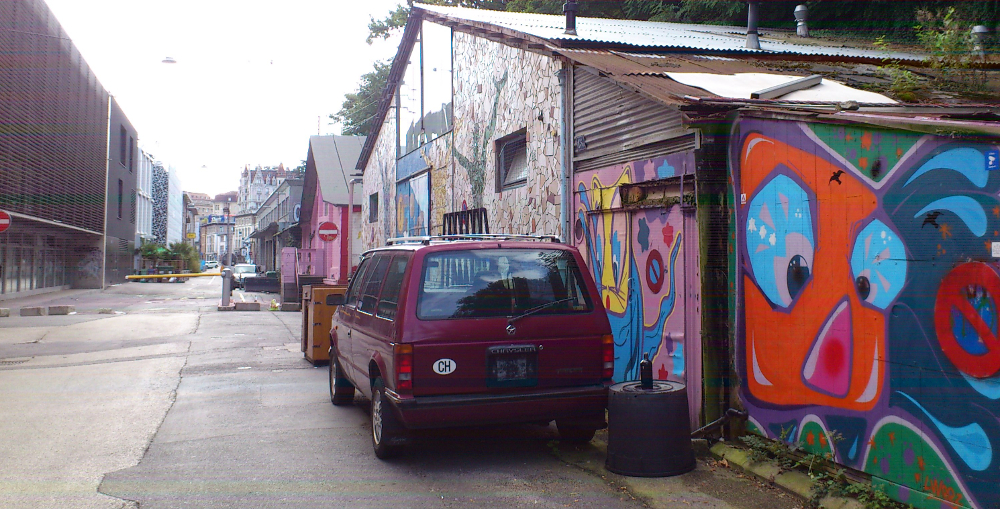
\includegraphics{img/BlumerSchuldt02.jpg}
\caption{Flon, situation 2014. On the right the last remainders of the
\enquote{old} Flon-Flon of the 1990s, on the left the backside of the
renovated buildings. The barracks on the right will be demolished, if
the \enquote{maison du livre et du patrimoine} will be build instead.}
\end{figure}

\subsection{The Place de la Riponne}\label{the-place-de-la-riponne}

As mentioned before, the Place de la Riponne is just one metro station
further up the hill from the neighborhood of Flon, surrounding together
with the Flon the economic most important parts of the city of Lausanne.
The spacious place is marked by the Palais de Rumine, which hosts the
Musée des Beaux-Arts, the Cantonal Library and other cultural
institutions. During the last decades, the place has lost its reputation
as cultural center, due to different innercity movements, such as the
Hotel Mövenpick, which moved to the neighborhood of Ouchy at the Lac
Léman, or the closing of the cinema Romandie, once the biggest cinema in
the city, which, after a transformation into a club, moved to a new
location next to the Flon. (City of Lausanne 2003)

For the last decade, local journals mostly mentioned the Riponne in a
negative manner, mainly because of the open drug scene. This scene may
be a result of the economic re-animation of the Flon and one could
assume that the drug users, one of the socially most vulnerable groups,
installed themselves on the Riponne, after having been repulsed as one
of the first groups by the ongoing gentrification process on the Flon.
Today, the open drug scene at the Riponne contains about 50 to 80
persons, organized in different groups, loosely oriented by perceived
ethnic characteristics, and constantly changing its different
\enquote{locations} on the place itself. In 2007, the city of Lausanne
tried to open a public injection room. After a very aggressive debate,
the population rejected the proposal in a public vote with a result of
54.6\%. (RTS 2007, Kraushaar 2012) Today, a mobile bus called
\enquote{Distribus}, operated for the social-work foundation
\enquote{Accueil à Bas Seuil} offers first aid, information and exchange
of sterile material for the described target group. There is a helping
infrastructure in place for the drug users and even if they are
described from the outside as \enquote{dangerous to everyone}, mostly
towards children, the groups generally remain in their own community and
solve the problems on their own. (Zehr 2014; see also Naegler 2012 for
nearly the same discussions in Hamburg.)

Still, the emptiness and wasted space of the place, which apparently
fosters the open drug scene, turns the place into a blemish of urban
planning. At the beginning of 2011, a proposal for a cultural
re-animation of the Riponne including a new cultural center with a
public library, has been announced by the minister of culture.
(Cordonier 2011) When she left the local politics shortly after this
last announcement, the project disappeared from the public attention and
apparently nothing happened. Only a few months later, another local
politician submitted a so called \enquote{Postulat}, a parliamentary
initiative, which asked the city for a sustainable solution of the
South-East of the place, where the majority of the drug users was
situated at this time. (Laurent 2011) As a direct answer, a few months
later another Postulat asked for the protection of the Northern part of
the place, as well. (Blanc 2011) Both initiatives were in the interest
of several shop and cafe owners within this area. According to them, the
hygienic conditions and security situation was intolerable and the
repeating conflicts within the drug using groups kept customers away. As
a last action, a petition with 1.435 signers, collected and submitted to
the communal council by a pub owner at the Northern end of the place
(Oberti 2011), turned the interest of the media to the Riponne and
nearly forced the local politics to find an appropriate solution. (RTS
2011) During the upcoming year, nothing really concrete in direction to
a cultural re-animation happened. The media attention was mostly turned
to another socially difficult area, not far away from the Place de la
Riponne, where the open drug scene, prostitution and homelessness
clashed with the inhabitants of an economic better-off quarter. (Barata
2012) In autumn 2012 and spring 2013, media wrote about violent
conflicts at the Riponne. (Détraz \& Giroud 2012, Maspoli 2013) As
Géraldine Morel argues, this growth of violence can be explained by the
fact that the drug users and homeless people started to feel attacked
themselves, because the number of present players, the rise of drug
prices, and the constant tension between vendors and buyers increased.
(Morel 2013) They felt that the space they could use for themselves
became smaller and smaller.

It was in spring 2014, when the city of Lausanne announces several
cultural actions, which took place during summer of the same year. (City
of Lausanne 2014) Soon afterwards, mobile snack bars are installed at
the Southern end of the place, one of the meeting points of the drug
users. Then, in the context of the cultural intervention project
\enquote{Lausanne Jardin 2014}, flower checks at free disposal were
installed at the Riponne as well as other places in the city which
should have been watched after by the marginals (De Paola 2014). An
ephemeral restaurant/bar, the \enquote{Café Grenette}, was installed at
the Northern end of the place, which offered, besides open and free
sitting opportunities, cultural activities, such as concerts, lectures
and activities for children. The concept included a mobile branch of the
public library of Lausanne in a container offering books and open-air
reading opportunities.\footnote{It has to be mentioned, that temporary
  or, rather connected to the topic of gentrification, \enquote{pop-up}
  branches of public libraries are not an unusual concept in
  Switzerland. Especially in the summer, library branches in parks,
  public pools, and other public or \enquote{tourist} places are quite
  common.} This project lasted the entire summer and ended in October
2014. (Rohrer 2014)

\begin{figure}[htbp]
\centering
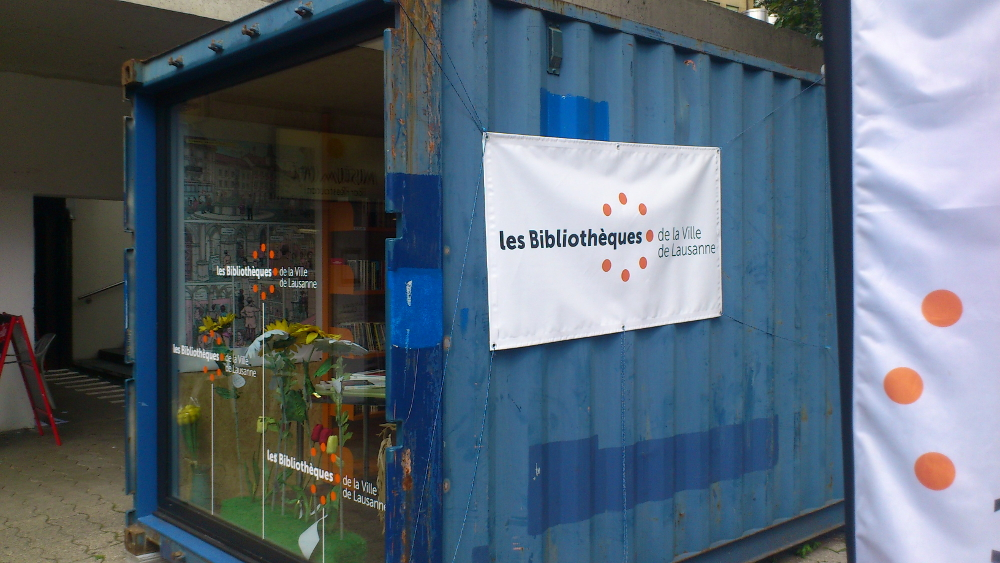
\includegraphics{img/BlumerSchuldt03.jpg}
\caption{The container of the branch of the public library at the Place
de la Riponne.}
\end{figure}

\begin{figure}[htbp]
\centering
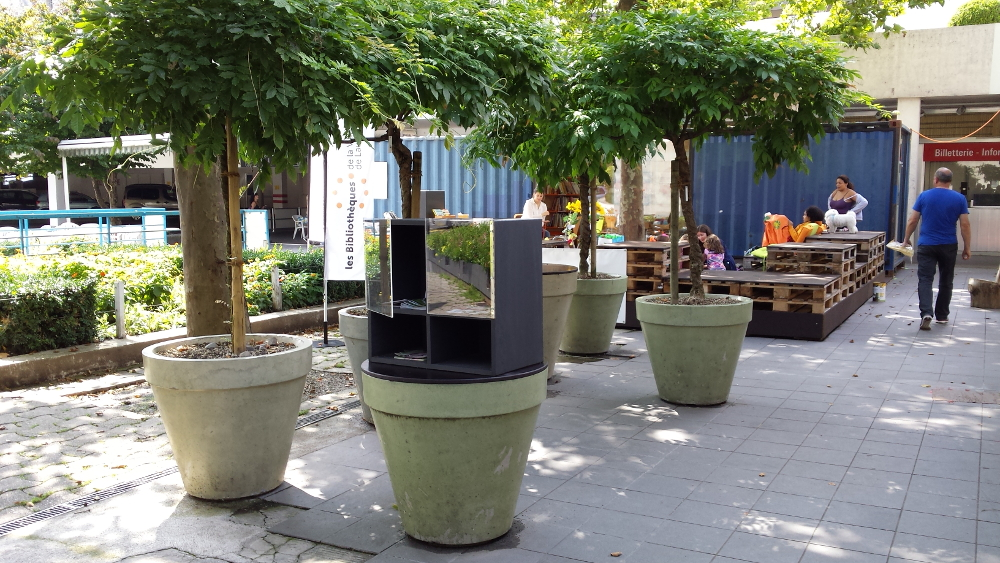
\includegraphics{img/BlumerSchuldt04.jpg}
\caption{A panorama of the public library container and the reading
possibilities in front of it. The small box in the front contains
information for free use.}
\end{figure}

\begin{figure}[htbp]
\centering
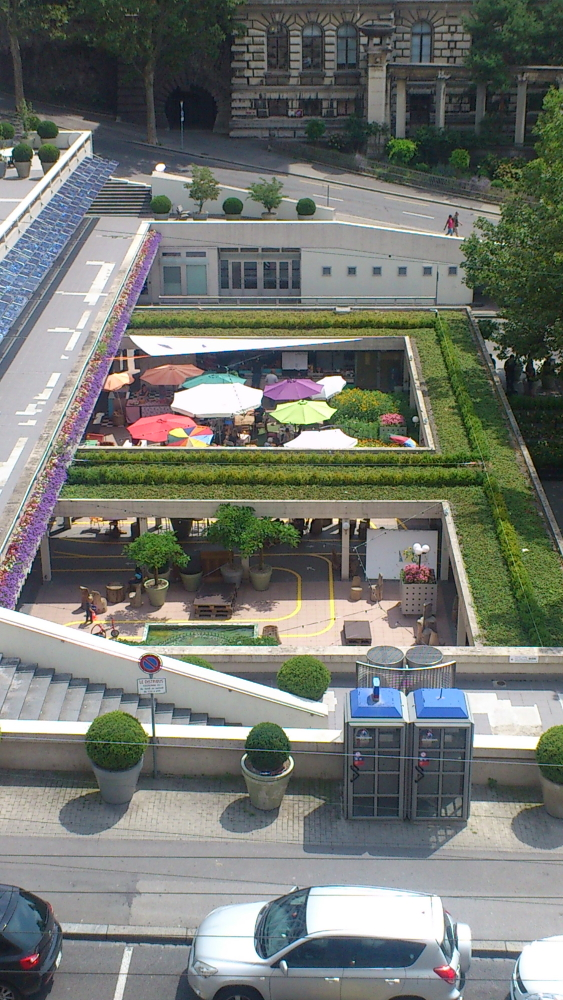
\includegraphics{img/BlumerSchuldt05.jpg}
\caption{A birds-eye view of the Café Grenette.}
\end{figure}

All these activities were taken in order to permit a better mixture
between the social vulnerable groups and better situated social groups,
as the local politics claimed. (De Paola, Cachin 2014) They are a good
example for how gentrification takes place. In Holms model, the Riponne
was suited for gentrification during a period of more than ten years,
meaning: in the first phase of gentrification. Even if it is not clear
how this process started, probably the upgrading of the Flon into the
third phase of gentrification around the year 2000 played an important
role. The Riponne now seems entering the second phase of gentrification,
where pioneers emerge in cities everyday picture, where young, hip and
wealthy people come by and make use of their offers, whereas the social
vulnerable groups such as the drug users and drug sellers are expelled
slowly. In the case of the Riponne, a forced expulsion in order to
repress the open drug scene is visible in the mobile snack bars at the
Southern part of the place, the Café Grenette and the public library
branch at the Northern end, and even in a more noticeable police
involvement. (De Paola 2014, Cachin 2014)

It is a question of time, how the Riponne will develop and if the
activities really continue into a full flown gentrification process. As
described before, gentrification is a process, not an automatism. Until
now, the case of the Riponne remains interesting, because the whole
revitalization process is apparently targeted to make the open drug
scene disappear, but until now it only led to a position shift of the
scene within the place. The \enquote{problem} seems not resolved so far,
but just relocated. But, at the same time, the Riponne became a new
in-place in Lausanne, where new shops have opened in previously closed
spaces. Moreover, different projects of renovation take place that could
solve problems the city have not been perceived as \enquote{important
enough} before.\footnote{DeSena (DeSena 2009) describes such a
  renovation project in Greenpoint, NY, were a rundown water park, that
  had been closed in the 1980s and was -- despite engagements of
  community groups -- left to rotten, had been renovated and opened
  again right at the time gentrification took of in Greenpoint, when
  working-class tenants left the neighborhood and middle-class people
  were moving in. She sees such projects, which take place right when
  gentrification starts -- the beginning of the second phase in Holms
  model -- as characteristic for such processes.}

As always, these processes of gentrification lead to the question, for
whom the space is reanimated. For everybody? For the city? For
\enquote{the right folks}? Or for the former users? For future
inhabitants? The open drug scene at the Riponne is only the most visible
group of users and actual tenants which now live in a new in-place with
rising rents and a new everyday culture. Is this good for them?

\section{The role of public libraries in
gentrification/revitalization}\label{the-role-of-public-libraries-in-gentrificationrevitalization}

The text will now turn to the public libraries and their role in the
described processes at the Flon and the Riponne.

First, the case of the Flon. As mentioned, this area can be described
now as being in the third phase of gentrification. In 2012 a competition
for architectural concepts for a \enquote{maison du livre et du
patrimoine} was proclaimed by the city of Lausanne. (Ville de Lausanne,
direction des travaux service d'architecture 2012) This house should be
placed at the edge of the Flon, right where the last remainders of the
second phase of gentrification can be found. If opened, it will be the
host of a youth library, a public library, the city archives, and the
historical comic collection of the city. As already mentioned, this
building could be interpreted as the last brick in the redevelopment
process of the Flon. This should not be underestimated. The city did not
choose anything for this last stone, but a cultural institution like the
library, which has a standing in the public as a place for everybody.
But who is this \enquote{everybody}? The Flon now is a space for
commercially oriented businesses and the people who are attracted by
those businesses, which is not the whole population of the city.

Secondly, in the case of the Place de la Riponne, the temporary Café
Grenette included a branch of the city's public libraries. This small
branch was tailored to children and their parents. The collection
contained mainly printed materials for children (picture books, first
reader material, comics etc.). Although the library itself didn't
announce anything on the concept and program of this specific branch, it
can be observed that especially on weekends this offer was used quite
strongly by young families. Again, this should not be underestimated.
Once more, the library was chosen as part of a process that could be
described as gentrification. Several other solutions would have been
possible. It could be asked, again, for whom this library is useful and
for whom not. Apparently the open drug scene, which is a part of the
\enquote{Riponne culture}, is not the target group, but a group that
previously has not been part of this culture. Nonetheless, this should
not be understood as a critique against the library itself. It is
without a doubt an important task to provide some offers for children
and their parents. It is just, as gentrification itself, a complex
situation.

These two libraries are not a seldom exception. Any deep research into
actual concepts of redevelopment of urban space provide examples for the
use of libraries within. When cities and other stakeholders reflect on
strategies to revitalize impoverished urban space, libraries turn up as
parts of these strategies again and again. (Lees, Slater \& Wyly 2008)
There could be different reasons for this, but it could be assumed that
the reputation of public libraries as cultural spaces open to all is an
important reason. Again, the case of Riponne provides an example for
this phenomenon. As mentioned before, already in 2011 a local politician
formulate a strategy for the reanimation of the place and included a
public library. (Cordonier 2011)

These two examples led to several open questions regarding the role of
libraries within such urban revitalization processes. Some of the most
striking ones are presented as follow, intended to be starting points
for discussions within the library community.

\begin{itemize}
\item
  It is self-evident that libraries should have an idea about the
  processes that happen around them, such as the ones which have been
  described in this text as gentrification. Obviously, this topic has
  become important in recent societal debates for a good reason. The
  question is, if libraries are aware of their participation in this
  processes, no matter if in active or passive ways? Libraries are, like
  the pioneers in the second phase of Holms model, in a conflicting
  position: They are both part and victim of those changes.
\item
  If libraries are always part of these changes, they could position
  themselves for or against them. The question is, if they should do so
  or not? Even if the answer is yes, it stands to discuss which position
  they should take. For instance: Should they foster urban development?
  Should they play an active role for the most socially vulnerable
  groups in the society? Or should they chose a middle ground? In any
  case, it should at least be discussed in an open way.
\item
  It is a matter of fact, if the libraries chose to stay passive, they
  will be utilized anyhow by the cities or investors. As gentrification
  has become part of societal debates, the decision to stay passive
  could mean to act against the interests of a part of the population.
  Again, this is a complex question and libraries can not escape this
  situation.
\item
  Should libraries be concerned with the effects of gentrification for
  the whole city? Usually, if one area becomes gentrified, another one
  impoverishes. People who leave a gentrified area, often don't leave
  the town, but look for a new space within city limits. Can libraries
  integrate these changes into their long-term strategies and if so,
  how?
\item
  As gentrification is an important debate in the society, libraries
  also can define themselves as information centers. Being a democratic
  institution, libraries can present facts and different positions on
  this topic and become a place of public debate. This may not be
  reduced to the distribution of handouts of different interest groups,
  but can include, for instance, discussion rounds, workshops on the
  change of urban space around the library, or exhibitions. But should
  libraries do so?
\end{itemize}

\section{Résumé: As cities change, libraries can not choose to
stand
aside}\label{ruxe9sumuxe9-as-cities-change-libraries-can-not-choose-to-stand-aside}

Public libraries can't escape the development of the cities they are in.
In recent years, projects of revitalization of urban space have become
re-interpreted as gentrification, whereas gentrification is perceive as
a complex process, with negative and positive effects. On the one hand,
gentrification, especially in the second phase, is seen as a rise of
cultural possibilities and a new life for former impoverished areas. But
on the other hand, gentrification became a word for displacement of poor
and socially vulnerable groups by better-of people of the middle class
and, in the third phase, a synonym for the commercialization of former
interesting urban spaces. Furthermore, it is, in some way, a paradox
process, because the people who seem to initiate it usually don't want
to cause the negative effects mentioned above.

Here Lausannes situation and two of its neighborhoods have been used to
discuss this process in light of the involvement of public libraries.
Because the concept of gentrification is apparently not yet a topic of
discussion in the library community, it took a long introduction for the
core subject of the text. This is common for topics which arise as new.
Anyhow, the text also made it clear that libraries are part of this
process, no matter what. Therefore this article can be seen as a first
contribution to a necessary discussion, beyond the case of Switzerland,
as gentrification today is a process observed in all of the countries of
the Global North. (Less, Slater \& Wyly 2008)

\section{Literature}\label{literature}

Alonso-Provencio, Marta, and Antonio Da Cunha. \enquote{Qualification de
lèspace public, commerce et urbanisme durable: notes sur le cas
lausannois}. \emph{Revue Géographique de l'Est} 53, Nr. 3--4 (2013):
1--16.

Andres, Lauren. \enquote{Temps de veille de la friche urbaine et
diversité des processus d'appropriation: la Belle de Mai (Marseille) et
le Flon (Lausanne)}. \emph{Géocarrefour} 81, Nr. 2 (2006): 159--66.

Andres, Lauren, and Boris Grésillon. \enquote{Cultural brownfields in
European cities: a new Mainstream object for cultural and urban
policies}. \emph{International Journal of Cultural Policy} 19, Nr. 1
(2013): 40--62. doi:10.1080/10286632.2011.625416.

Anonymous. \enquote{Le Flon secret?: Une galerie}. \emph{gazette du
flon}. October 1989.

Barata, Andreia et al. \enquote{Passage Riant-Mont: pas de zone de
‚non-droit`.} Blog. Lausanne Tunnel\emph{.} Accessed 7 september 2014.
\url{http://lausannetunnel.wordpress.com/}.

Bonal, Keriam, and Sigmar Gude. \enquote{Gentrifizierung oder Wiederkehr
der Wohnungsnot?: Sozialstrukturelle Entwicklungstendenzen in Berliner
Innenstadtwohngebieten}. In \emph{Reclaim Berlin: Soziale Kämpfe in der
neoliberalen Stadt}, edited by Andrej Holm, 27--49. Berlin; Hamburg:
Assoziation A, 2014.

Cachin, Jérôme. \enquote{Lausanne veut «rendre» la place de la Riponne
aux habitants}, 11 april 2014.
\url{http://www.laliberte.ch/news/regions/vaud/lausanne-veut-rendre-la-place-de-la-riponne-aux-habitants-233427}.

Chesnay, Catherine, Céline Bellot, and Marie-Ève Sylvestre.
\enquote{Judiciarisation des personnes itinérantes à Québec: une
géographie des pratiques policières répressives au service de la
revitalisation}. \emph{EchoGéo} 28, Nr. avril / juin (2014): 2--17.

Cordonier, Gérald. \enquote{Lausanne a un plan d'enfer pour redessiner
la Riponne}. Journal. \emph{24 heures}, 18 february 2011.
\url{http://archives.24heures.ch/vaud-regions/actu-vaud-regions/lausanne-plan-enfer-redessiner-riponne-2011-02-18}.

De Paola, Vicky. \enquote{Lausanne veut rendre la place de la Riponne à
ses habitants}. \emph{Les News, Blog de la Rédaction, Rouge FM, Yes.fm},
10 april 2014.
\url{http://blogredaction.rougefm.com/actu/lausanne-veut-rendre-la-place-de-la-riponne-a-ses-habitants/}.

Dép. Culture, Sports, Patrimoine, Travaux, Ville Lausanne.
\enquote{Préavis 2003/3: Place de la Riponne 10 - Rénovation et
transformation du cinéma Romandie}, 23 januar 2003. .

DeSena, Judith N. \emph{Gentrification and Inequality in Brooklyn: The
New Kids on the Block}. Lanham: Lexington Books, 2009.

Détraz, Alain, and Giroud, Fanny. \enquote{Violente bagarre à la
Riponne}. Tribune de Genève, 19 September 2012.
\url{http://www.tdg.ch/suisse/faits-divers/violente-bagarre-riponne/story/17584527}.

Fondation ABS. \enquote{Le Distribus}. Accessed 30 August 2014.
\url{http://www.fondationabs.ch/Distribus.htm}.

Godsil, Rachel D. \enquote{The Gentrification Trigger: Autonomy,
Mobility, and Affirmatively Furthering Fair Housing}. \emph{Brooklyn Law
Review} 78, Nr. 2 (2013): 319--38.

Hae, Laam. \emph{The Gentrification of Nightlife and the Right to the
City: Regulating Spaces of Social Dancing in New York}. Routledge
Advances in Geography. New York; London: Routledge, 2012.

Heinen, Christina M. ``*Tief in Neukölln``: Soundkulturen zwischen
Improvisation und Gentrifizierung in einem Berliner Bezirk*. Studien zur
Popularmusik. Bielefeld: transcript Verlag, 2013.

Holm, Andrej. \enquote{Gentrification in Berlin: Neue
Investionsstrategien und lokale Konflikte}. In \emph{Die Besonderheit
des Städtischen: Entwicklungslininen der Stadt(soziologie)}, edited by
Heike Hermann, Carsten Keller, Rainer Neef, and Renate Ruhne, 213--32.
Wiesbaden: VS Verlag für Sozialwissenschaften, 2011.

---------. \enquote{Reclaim Berlin}. In \emph{Reclaim Berlin: Soziale
Kämpfe in der neoliberalen Stadt}, edited by Andrej Holm, 7--24. Berlin;
Hamburg: Assoziation A, 2014.

Kraushaar, Beat. \enquote{Schweiz am Sonntag - Die offene Drogenszene
von Lausanne}. \emph{Schweiz am Sonntag}. Accessed 30 august 2014.
\url{http://www.sonntagonline.ch/ressort/nachrichten/2418/}.

Kullmann, Katja. \emph{Rasende Ruinen: Wie Detroit sich neu erfindet}.
edition suhrkamp digital. Berlin: Suhrkamp, 2012.

Lees, Loretta, Tom Slater, and Elvin Wyly. \emph{Gentrification}. New
York: Routledge, 2008.

Lévy, Jacques. \enquote{Der Raum als öffentliches Gut}. \emph{Forum
Raumentwicklung} 41, Nr. 3 (2013): 25--28.

Maspoli, Par Philippe. \enquote{Lausanne: Le marché de la Riponne
souffre de l'insécurité}. \emph{24 heures}, 19 april 2013.
\url{http://www.24heures.ch/vaud-regions/lausanne-region/Le-marche-de-la-Riponne-souffre-de-l-insecurite-/story/21715145}.

Morel, Géraldine. \enquote{Marginalité urbaine, espace public et usage
de droguue: Lausanne, automne 2012}, 31 january 2013.
\url{http://www.chanvre-info.ch/info/fr/Marginalite-urbaine-espace-public.html}.

Naegler, Laura. \emph{Gentrification and Resistance: Cultural
criminology, control, and the commodification of urban protest in
Hamburg}. Hamburger Studien zur Kriminologie und Kriminalpolitik 50.
Berlin: LIT Verlag, 2012.

Prince, Sabiyha. \emph{African Americans and Gentrification in
Washington, D.C.: Race, Class and Social Justice in the Nation's
Capital}. Urban Anthropology. Farnham; Burlington: Ashgate, 2014.

Rohrer, Joshua. \enquote{{[}Lettre aux voisins de Riponne{]}}, July
2014.

RTS. \enquote{Couleurs locales - VD: la place de la Riponne à Lausanne,
autrefois lieu de rassemblement convivial, est aujourd'hui le lieu de
rendez-vous des dealers, toxicomanes et autres marginaux}. Téléjournal.
\emph{rts.ch}, 19 december 2011.
\url{http://www.rts.ch/video/info/couleurs-locales/3661310-vd-la-place-de-la-riponne-a-lausanne-autrefois-lieu-de-rassemblement-convivial-est-aujourd-hui-le-lieu-de-rendez-vous-des-dealers-toxicomanes-et-autres-marginaux.html}.

Sassen, Saskia. \emph{The global city: New York, London, Tokyo}. 2.
edit. Princeton, NJ; Oxford: Princeton University Press, 2001.

Schuetz, Jenny. \emph{Do Art Galleries Stimulate Redevelopment?}.
University of Southern California Lusk Center, 2013.
\url{http://ssrn.com/abstract=2305430}.

Stadt Zürich Präsidialdepartement. \enquote{Deutlicher Anstieg der
Leerwohnungszahl}. Press release. Zürich, 6 august 2014.
\url{https://www.stadt-zuerich.ch/prd/de/index/ueber_das_departement/medien/medienmitteilungen/2014/august/140806a.html}.

Stock, Miriam. \emph{Der Geschmack der Gentrifizierung: Arabische
Imbisse in Berlin}. Urban Studies. Bielefeld: transcript, 2013.

Téléjournal RTS. \enquote{le 19:30 - Local d'injection à Lausanne: le
peuple dit clairement non}. Téléjournal. \emph{rts.ch}, 8 july 2007.
\url{http://www.rts.ch/video/info/journal-19h30/1488259-local-d-injection-a-lausanne-le-peuple-dit-clairement-non.html}.

Terrin, Jean-Jacques. \enquote{La ville et ses créateurs / The City and
its creators}. In \emph{La ville des createurs / The city of creators:
Berlin, Brimingham, Lausanne, Lyon, Montpellier, Montréal, Nantes,
Montréal}, edited by Jean-Jacques Terrin, 12--27. Marseille: Editions
parenthèses, 2012.

Ville de Lausanne. \enquote{Bulletin du Conseil communal Lausanne} 125e
année, No 6 (27 september 2011).
\url{http://www.lausanne.ch/lausanne-officielle/conseil-communal/bulletins-du-conseil-communal/bulletins-2011/mainArea/00/links/01111/linkBinary/BCC_06_II\%20du\%2008.11.11_Voiblet_spb.pdf}.

---------. \enquote{Bulletin du Conseil communal Lausanne} 125e année ,
No 4 (27 september 2011).
\url{http://www.lausanne.ch/lausanne-officielle/conseil-communal/bulletins-du-conseil-communal/bulletins-2011/mainArea/00/links/0116/linkBinary/BCC_04_I\%20du\%2027.09.11_Voiblet.pdf}.

---------. \enquote{Bulletin du Conseil communal Lausanne} 126e année,
No 10 (17 january 2012).
\url{http://www.lausanne.ch/lausanne-officielle/conseil-communal/bulletins-du-conseil-communal/bulletins-2012/mainArea/00/links/019/linkBinary/Bulletin\%20du\%20Conseil\%20No\%2010-II\%20du\%2017.01.12\%20-\%20spblanches.pdf}.

---------. \enquote{Redynamiser la place de la Riponne: Conférence de
presse du 10 avril 2014}, 10 april 2014.
\url{http://www2.lausanne.ch/export/actualites/Next/serve.php?id=4211}.

Ville de Lausanne, direction des travaux service d'architecture.
\emph{Construction de la «Maison du livre et du patrimoine»
(bibliothèque et archives de la Ville de Lausanne): Rapport du Jury}.
Rapport du jury. Lausanne: Ville de Lausanne, 18 december 2012.
\url{http://www.lausanne.ch/lausanne-officielle/administration/travaux/architecture/concours/concours-archives/maison-du-livre-et-du-patrimoine/mainArea/00/col2/04/text_files/file0/document/RapJury_ConcoursVigie-Gonin_Final.pdf}.

Zuppinger, Urs. \emph{Luttes-ô-Flon: une reconversion urbaine
lausannoise mouvementée de 1984 à 2012}. Lausanne: Éditions d'En Bas,
2012.

Zehr, Angelo. \enquote{Uf de Gass: Ein Stück Lebensschule,} 2014.
\url{http://www.uf-de-gass.ch/}.

%autor
\begin{center}\rule{0.5\linewidth}{\linethickness}\end{center}

\textbf{Eliane Blumer} is a research fellow at the Data Lifecycle
Management Project at the University of Geneva and mandatee for
continuing education at the Swiss library association BIS.

\textbf{Dr.~Karsten Schuldt} is a research fellow at the Swiss Institute
of Information Science at the University of Applied Sciences in Chur and
editor of LIBREAS. Library Ideas. Both live and work in Berlin, Chur,
Geneva and Lausanne.

\end{document}
